\subsection{Initial analysis}
First, we decided to explore our data with respect to severity, which is useful for our analysis.
\begin{figure}[htpb!]
	\centering
	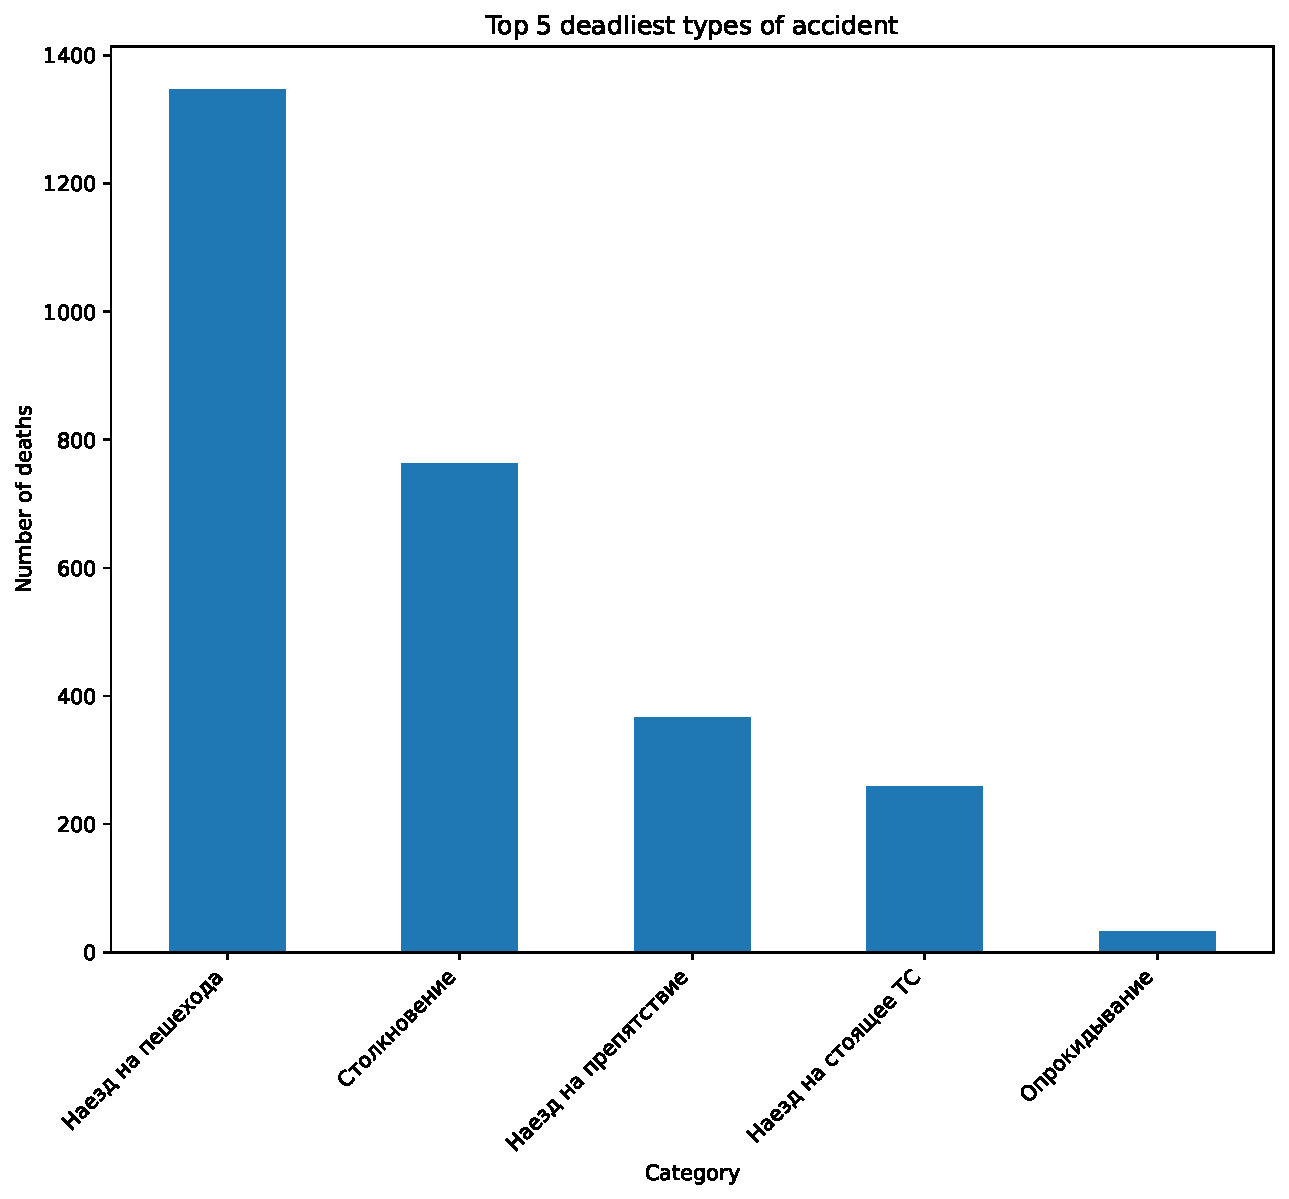
\includegraphics[width=0.5\textwidth, scale=0.4]{../imgs/pdf_files/top5deaths.pdf}
	\caption{\textbf{Top categories by deaths}}
	\label{fig:top5d}
\end{figure}
We can see from figure \ref{fig:top5d} that most of the deaths occur when pedestrians are involved, next deadliest are crashes, obstacle encounter,
crashes with non-moving vehicles, overturns. Nothing surprising. We get similar results for injuries:
\begin{figure}[H]
	\centering
	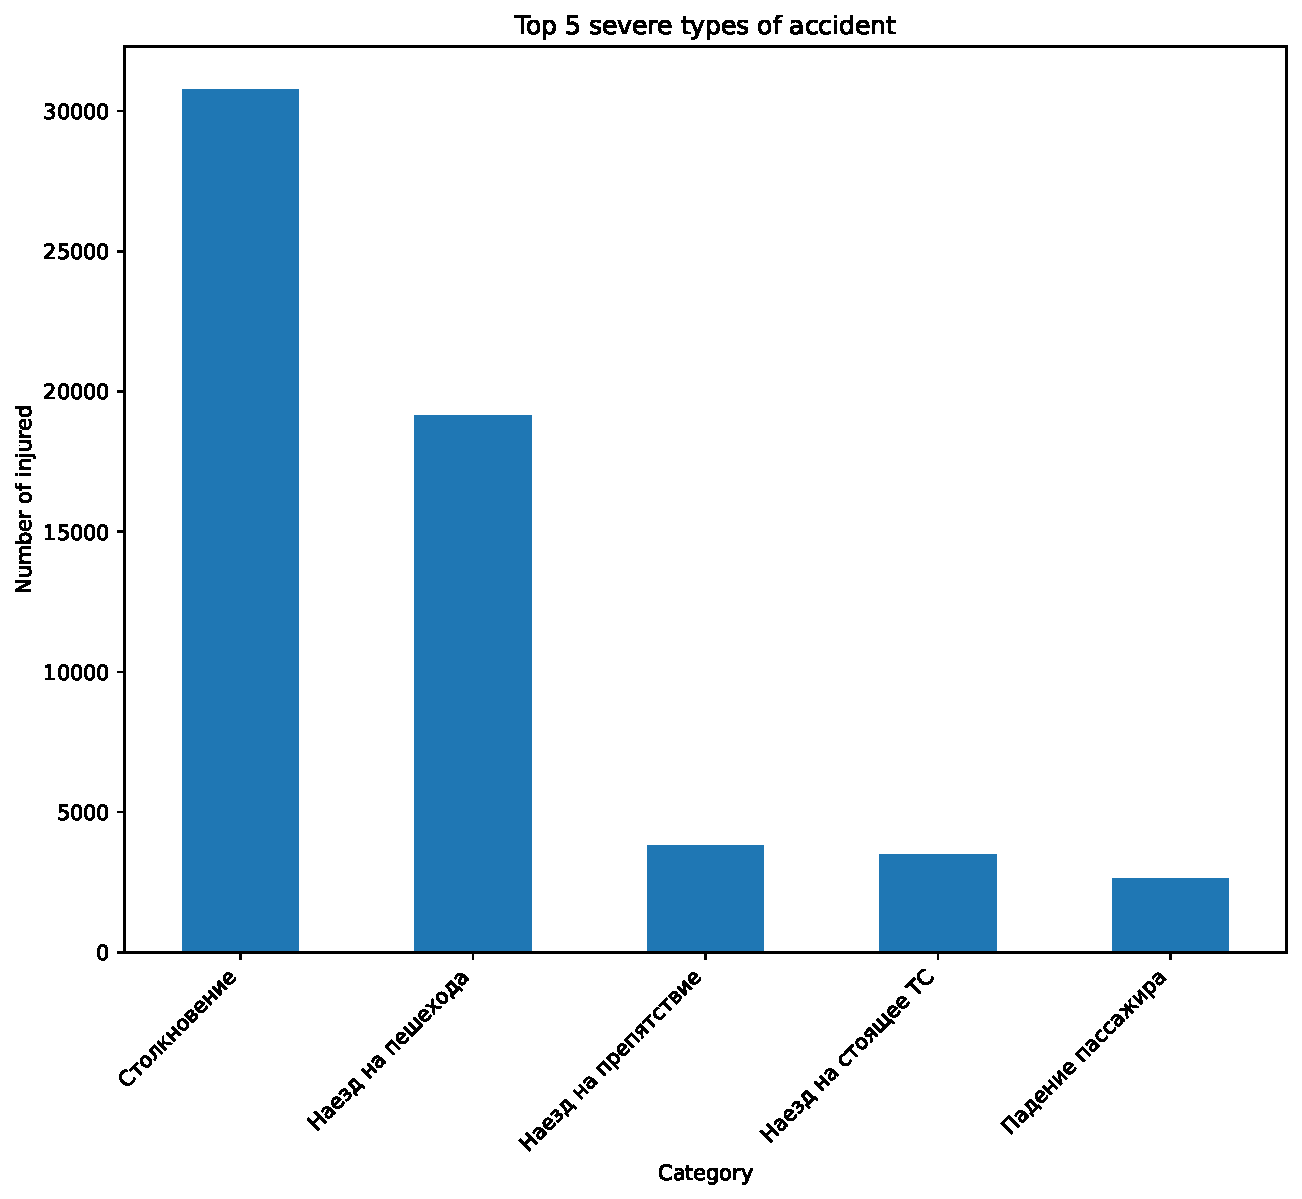
\includegraphics[width=0.5\textwidth, scale=0.4]{../imgs/pdf_files/top5injuries.pdf}
	\caption{\textbf{Top categories by injuries}}
	\label{fig:top5inj}
\end{figure}
\noindent
 Most injuries occur during crashes, pedestrian and obstacle encounters, crashes with non-moving vehicles,
falls of passengers.
Interestingly, if we count number of deaths with respect to total participants by category of accident, we get the following results:
\begin{table}[H]
	\centering
	\label{tab:prob_death}
	\begin{tabular}{|c|c|}
		\hline
		Category & $P_{\text{death}}$ \\
		\hline
		Hitting maintenance worker & 0.23 \\
		\hline
		Crash into ditch & 0.14 \\
		\hline
		Hitting other & 0.12 \\
		\hline
		Hitting police officer & 0.09 \\
		\hline
		Running over animals & 0.09 \\ 
		\hline
		Obstacle encounter & 0.09 \\
		\hline
		Overturn & 0.05 \\
		\hline
		Other type of accident & 0.05 \\
		\hline
	\end{tabular}
	\caption{\textbf{Top 8 Probability of death with respect to accident}}
\end{table}
\noindent
The high mortality rate is not surpising. There are relatively few participants in these types of accidents (less than 130), except obstacle encounter.
All of these events are quite similar in terms of that they mostly happen on motorways, where speeds are high and thus crashes are more lethal when
they occur. However, as we saw from figure \ref{fig:top5d} most deaths occur in habited areas. \\
\subsection[Clusterization]{Clusterization\footnote{\href{https://github.com/isdevnull/cw3/blob/dev/clusters.ipynb}
{https://github.com/isdevnull/cw3/blob/dev/clusters.ipynb}}}
Our data possesses geospatial properties, that is why we decided that it would be nice to explore potentially dangerous areas. There are just too
many accidents in Moscow, so it may seem that they cover almost all of the streets and motorways and in fact it is absolutely true. However,
we can employ density-based clusterization technique to select only those spots on the map that are most dense in terms of car accidents. To do that
we use DBSCAN \cite{DBSCAN}, which can select clusters of complex form, depends only on a few hyperparameters which are easily interpretable.
\begin{figure}[H]
	\centering
	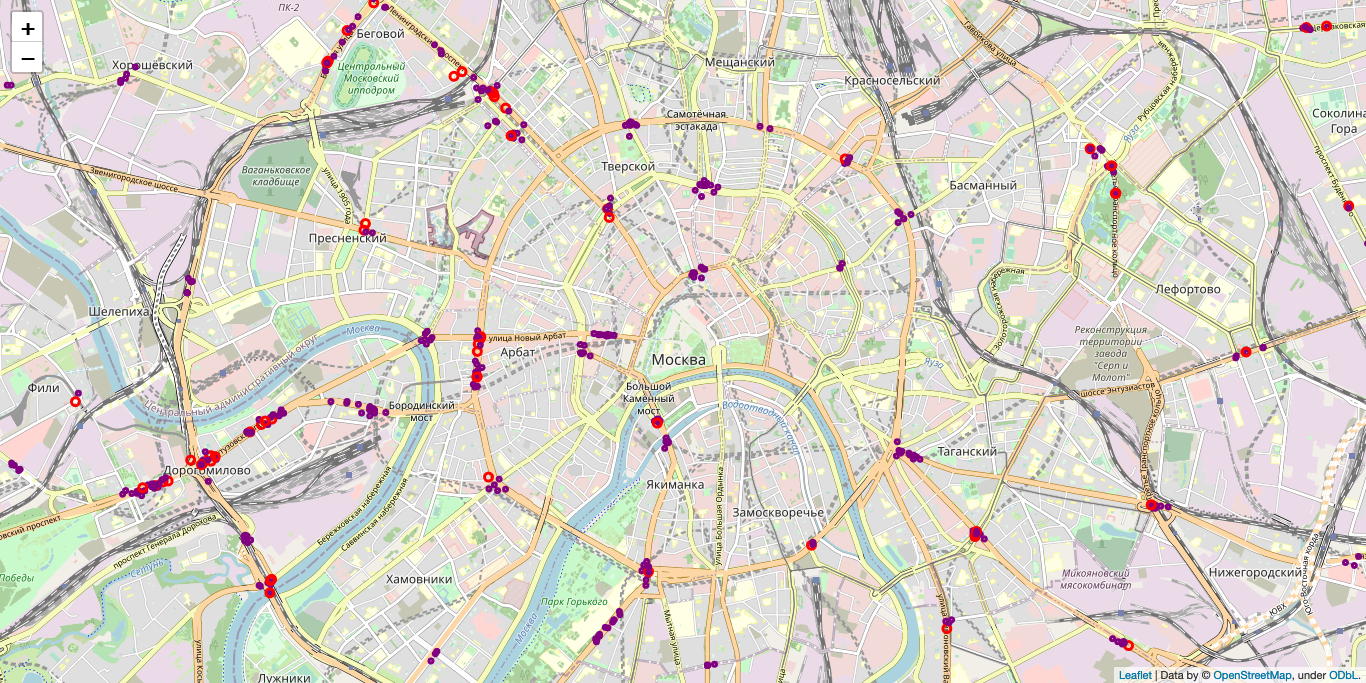
\includegraphics[width=0.8\textwidth]{../imgs/png_files/msc_problem_regions.png}
	\caption{Clusterizaion with U=$\frac{0.1}{6371}$, N=$15$; red points – deadly accidents, purple – heavy severe}
	\label{fig:DBSCAN}
\end{figure}
These are neighbourhood of a point – $U$ and number of members – $N$ to be considered as core point.
Due to Earth being spherical we use Haversine distance and
transform our geospatial data to radians, thus neighbourhood $U$ in our case is distance between multiple accidents and core samples are defined as
those that have $N$ accidents around it, scattered in time. When DBSCAN selects $M$ clusters, we firstly delete noise points, then we do not
distinguish between clusters, because we are only interested, in general, how problematic regions are distributed. We color accidents according
to their severity. The larger the $U$ hyperparameter the bigger the problematic regions and the more spreaded they are.
\subsection{Time Series Analysis}

Because we want to predict severity and it is a categorical variable, we assign labels from 0 to 2, ranging fron non-severe to lethal accidents.
